\documentclass[conference]{IEEEtran}
%\IEEEoverridecommandlockouts
% The preceding line is only needed to identify funding in the first footnote. If that is unneeded, please comment it out.
\usepackage{cite}
\usepackage{amsmath,amssymb,amsfonts}
\usepackage{algorithmic}
\usepackage{graphicx}
\graphicspath{{images/}}
\usepackage{textcomp}
\usepackage{xcolor}
\usepackage{hyperref}
\usepackage{fancyhdr}
\renewcommand{\headrulewidth}{0pt}
\pagestyle{fancy}
\lfoot{Does a higher quality of living contribute to a lower suicide rate?}
\cfoot{}
\rfoot{\thepage}
\usepackage[belowskip=-15pt,aboveskip=0pt]{caption}

\def\BibTeX{{\rm B\kern-.05em{\sc i\kern-.025em b}\kern-.08em
    T\kern-.1667em\lower.7ex\hbox{E}\kern-.125emX}}
\begin{document}

\title{Does a higher quality of living contribute to a lower suicide rate?\\
}

\author{\IEEEauthorblockN{Owen Prosser}
\IEEEauthorblockA{\textit{School of Computer Science} \\
\textit{University of Lincoln}\\
Lincoln, United Kingdom \\
14514822@students.lincoln.ac.uk}
}

\maketitle

\begin{abstract}
    Lorem ipsum dolor sit amet, consectetur adipiscing elit. Mauris feugiat felis nibh, id condimentum risus condimentum et. Sed id orci nec arcu convallis posuere. Aliquam orci arcu, viverra in posuere ac, luctus vitae nulla. Vivamus vitae consectetur sapien. Vivamus sodales id nisl lacinia imperdiet. Aenean fringilla massa dolor, id malesuada.
\end{abstract}

\begin{IEEEkeywords}
developed, developing, suicide
\end{IEEEkeywords}

\section{Introduction}
Life is very diffent in any of the different countries on Earth. One's country of Birth or Country of residence
has a huge impact on all aspects of one's life. This paper investigates the existance of a link between
the standard of living of a country and it's rate of suicide.Previosuly there has been little consensus on the issue
with 45\% of research finding a significant relationship between socio-economic factors and suicide rate, and 55\%
finding no relationship at all\cite{sui_systematic_review}.

\subsection{Motivation}
To discover if there is any link between Living Standards and Suicide rate which would be useful in aiding further
research into the other, more specific, causes. It has been shown that current state of the economy
has an impact on the suice rate when compared with historical data \cite{Suicides_2008-10}. This could result in more effective action being taken to combat this
issue and potentailly reduce the number suicides.

\subsection{Choice of Dataset}
The dataset for this paper was selected as it contained a wide set of detailed data on the subject.
It contains the data for around 117 countries from all over the globe and from all areas of the wealth and quality of living spectrum.
The dataset is also provided by a reliable source, the World Health Organisation (WHO).

\subsection{Research Hypothesis}
The Hypothesis for this paper was established by firstly analysing the dataset using descriptive statistics.
A total of six countries were selected for this paper with three on each end of the quality of living spectrum.
The top tree countries were selected based on the highest ``Social Progress Index’’ values of those countries contained within this dataset.
The ``Social Progress Index'' is based on three components, Basic Human Needs, Foundations of Wellbeing, and Opportunity\cite{high_standard_living}.
These are the Scandinavian countries, Sweden, Norway and the Netherlands.
The three lowest in the dataset are, Russia, Chile and Brazil.

The Histogram in Figure 1 shows that there is some correlation between the standard of living and the suiicde rate.
The two highest values of suicide per-capita are associated with two of the counties with the lowest standard of living.
This can justify further study into the hypothesis.
\newline
    \begin{figure}[b]
        \centering
        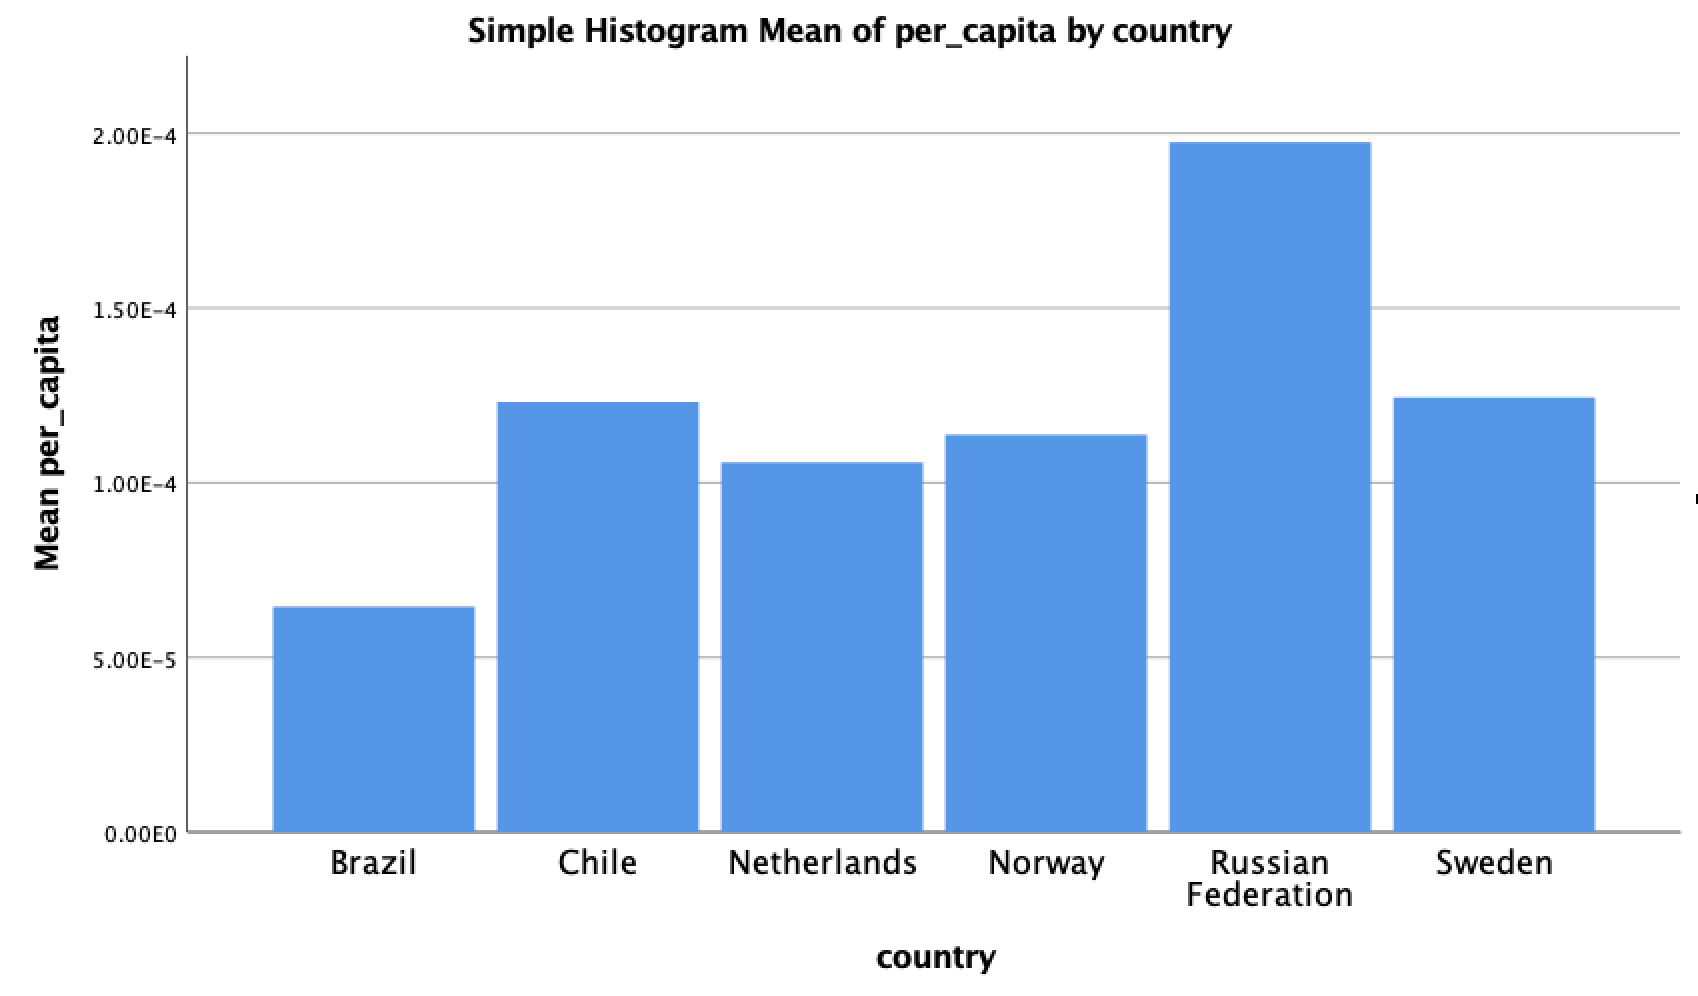
\includegraphics[width=0.4\textwidth]{percapita_bar}
        \caption{Histogram of the per-capita suicide rate of six countries.}
    \end{figure}

\section{Related Work}
``Suicide is the 15th leading cause of death worldwide, with over 75\% of suicides occurring in low-income and middle-income countries''\cite{sui_low_income}.
Vijayakumar, Lakshmi, et al evaluated the links between the effects of the Human Development Index (HDI) and examined the
``association between a range of socioeconomic factors and suicide rate''.
In this case the studied countries were classified based on their HDI value in 2003 \cite{Sui_in_developing}.

Linear regression has been used to investigate similar hypothesis, Chang et al used the teqnique to investigate a 
correlation between a rising suicide rate and the Southeast Asian economic downturn of 1997 \cite{SEAsia_sui}.
Linear Regressions are used to analyse the multi-variate dataset. A liner regression is a technique used to demonstrate the relationship between two scaler variables \cite{stats_models_book}. 
In this case it was used to ``examine the relationship between suicide rates, the economic crisis and other socio-economic variables''\cite{SEAsia_sui}.

One paper investigating a similar hypothesis used a Spearman Correlation to investigate a connection between suicide and gun ownership in geographic areas.
Spearman's correlation is a nonparametric measure which shows the relationship between two variables\cite{gun_sui}.
The technique of analysis could be applied to this particular hypothesis as the Spearman's Correlation relies on two varibles of scale type or one scale and one ordinal.
The varibles for this paper, Country and the per-capita suicide rate, are ordinal and scale allowing for this type of analysis to be conducted.

\section{Methodology}
The dataset was imported in full into SPSS. The first step was to remove the data which was not relevant to testing this hypothesis.
This was done using the ``Select Cases'' function in SPSS which allows for rows of the dataset to be deleted if they do not match a specified condition.
This left a subset of the initial dataset which contained the data for the countries to be analysed as explained in Research Hypothesis section.
The rows which were removed were those that the `Country' field did not match any of the six counties focused on in this paper.

Then the task was to find which types of statistical tests would be the most useful and appplicable to the dataset in question.
To do this it was necessary to establish if the data in the dataset was parametric or non-parametric.
This is done by looking at the distrobution of the data. If the data follows a normal distrobution is it parametric, otherwise it is non-parametric.
This result affects the statistical tests that can be applied to the dataset.
In this case the data is right-skewed this can been seen in Fig 2. This means that the data is non-parametric.

In this case the country variable is ordinal data as the countries are ranked in order of the expected standard of living in each (as covered in the `Research Hypothesis' subsection).
As the country information in the dataset contained the country names (strings) they needed to be processed before the data could be analysed in SPSS as it will only accept integer data for the anaysis.
The countries were ranked from one to six based on thier relative standard of living from the Social Progress Index.

Spearman's Correlation was used to investigate if there is a link between these two variables in this dataset.

    \begin{figure}[b]
        \centering
        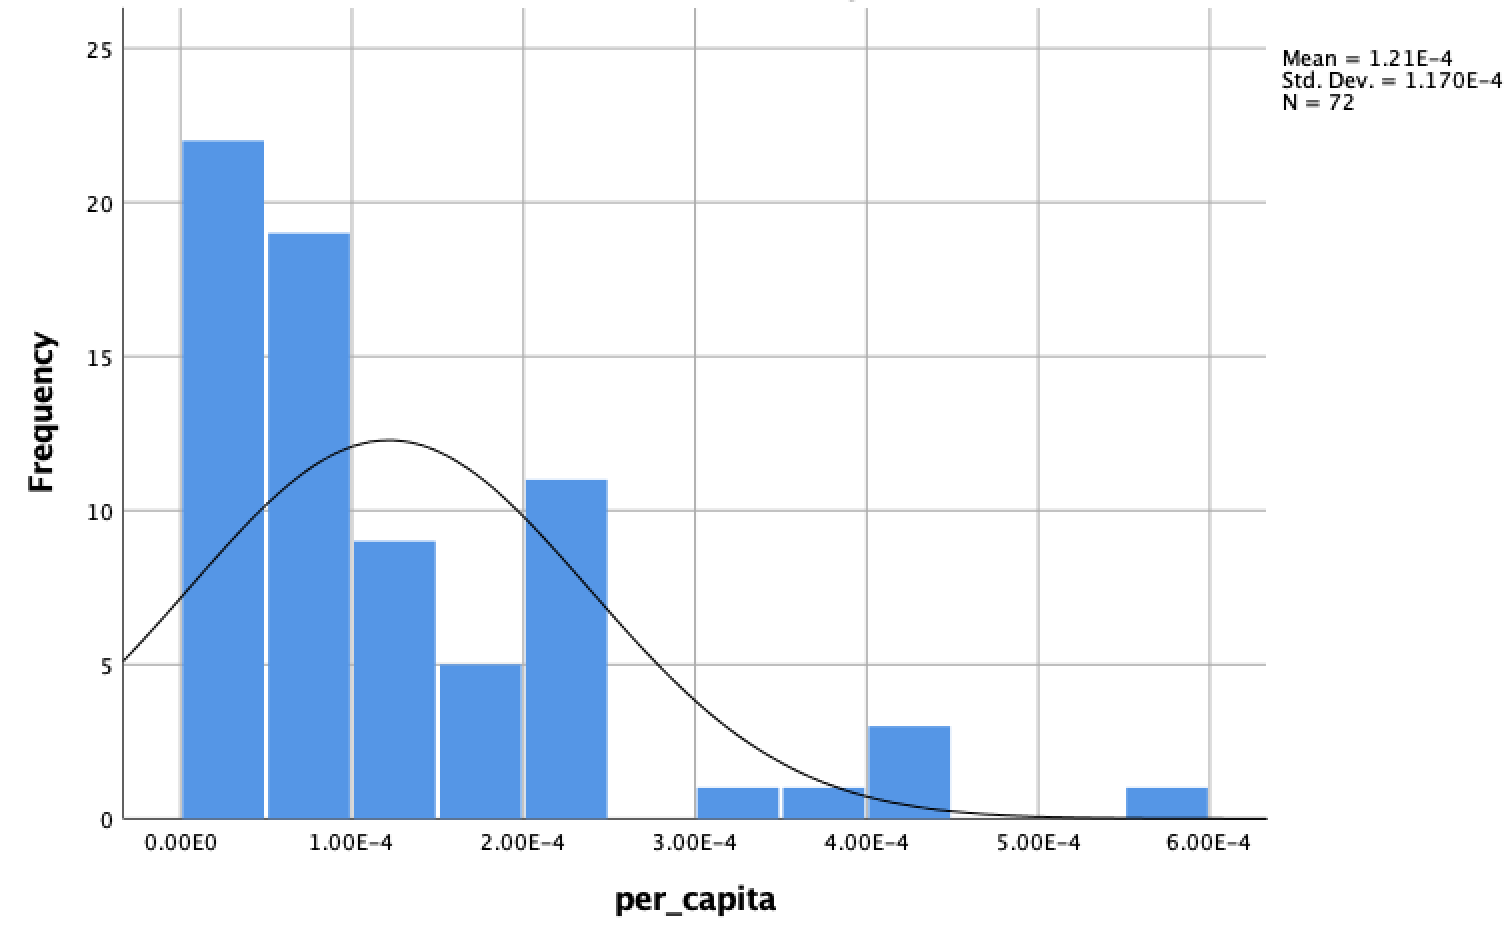
\includegraphics[width=0.45\textwidth]{skewed}
        \caption{The distrobution of data in the dataset.}
    \end{figure}

\section{Results}
The results of the analysis showed The results of the analysis showed The results of the analysis showed
\newline

\begin{figure}[b]
    \centering
    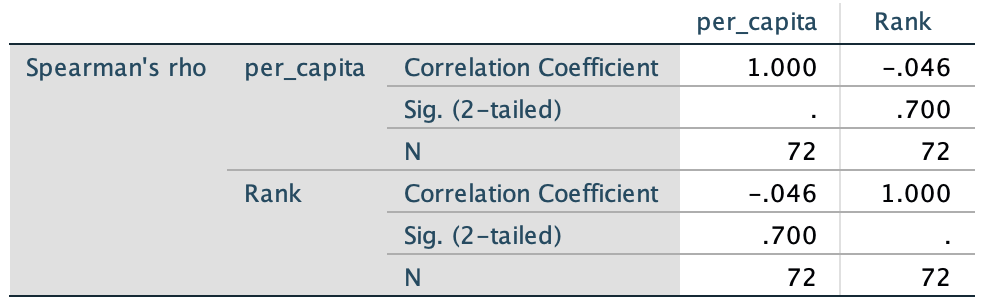
\includegraphics[width=0.45\textwidth]{spearmans}
    \caption{The results of the Spearman's Correlation.}
\end{figure}

\begin{table}[ht]
    \centering
    \caption{Descriptive Statistics}
    \begin{tabular}{| l | l | lll |}
    \hline
     Brazil&  Mean&  &  0.000065&   \\
     &  95\% confidence Interval&  Upper Bound&  0.000103&   \\
     &  &  Lower Bound&  0.000026&   \\
     Chile&  Mean&  &  0.000123&   \\
     &  95\% confidence Interval&  Upper Bound&  0.000201&   \\
     &  &  Lower Bound&  0.000046&   \\
     Netherlands&  Mean&  &  0.000106&   \\
     &  95\% confidence Interval&  Upper Bound& 0.000158&   \\
     &  &  Lower Bound&  0.000054&   \\
     Norway&  Mean&  &  0.000114&   \\
     &  95\% confidence Interval&  Upper Bound&  0.000161&   \\
     &  &  Lower Bound&  0.000066&   \\
     Russia&  Mean&  &  0.000197&   \\
     &  95\% confidence Interval&  Upper Bound&  0.000320&   \\
     &  &  Lower Bound&  0.000075&   \\
     Sweden&  Mean&  &  0.000124&   \\
     &  95\% confidence Interval&  Upper Bound&  0.000188&   \\
     &  &  Lower Bound&  0.000061& \\\hline
    \end{tabular}
    \end{table}

\section{Conclusion}

\subsection{Future Work}

\begin{thebibliography}{00}
%\bibitem{b1} G. Eason, B. Noble, and I. N. Sneddon, ``On certain integrals of Lipschitz-Hankel type involving products of Bessel functions,'' Phil. Trans. Roy. Soc. London, vol. A247, pp. 529--551, April 1955.
\bibitem{sui_systematic_review}Iemmi, Valentina, Jason Bantjes, Ernestina Coast, Kerrie Channer, Tiziana Leone, David McDaid, Alexis Palfreyman, Bevan Stephens, and Crick Lund. "Suicide and poverty in low-income and middle-income countries: a systematic review." The Lancet Psychiatry 3, no. 8 (2016): 774-783.
\bibitem{Suicides_2008-10} Barr, B., Taylor-Robinson, D., Scott-Samuel, A., McKee, M. and Stuckler, D., "Suicides associated with the 2008-10 economic recession in England: time trend analysis". Bmj, 345, p.e5142, 2012..
\bibitem{high_standard_living} M. Smith, ``The 19 countries with the highest standard of life'', Business Insider. New York, 2016.
\bibitem{sui_low_income} Iemmi, Valentina, Jason Bantjes, Ernestina Coast, Kerrie Channer, Tiziana Leone, David McDaid, Alexis Palfreyman, Bevan Stephens, and Crick Lund. "Suicide and poverty in low-income and middle-income countries: a systematic review." The Lancet Psychiatry 3, no. 8 (2016): 774-783.
\bibitem{Sui_in_developing} Vijayakumar, Lakshmi, et al. "Suicide in Developing Countries (1) Frequency, Distribution, and Association with Socioeconomic Indicators." Crisis 26.3 (2005): 104-111
\bibitem{SEAsia_sui} Chang, Shu-Sen, David Gunnell, Jonathan AC Sterne, Tsung-Hsueh Lu, and Andrew TA Cheng. "Was the economic crisis 1997–1998 responsible for rising suicide rates in East/Southeast Asia? A time–trend analysis for Japan, Hong Kong, South Korea, Taiwan, Singapore and Thailand." Social science \& medicine 68, no. 7 (2009): 1322-1331.
\bibitem{stats_models_book}Freedman, David A. Statistical models: theory and practice. Cambridge University Press, 2009.
\bibitem{gun_sui}Kaplan, Mark S., and Olga Geling.``Firearm suicides and homicides in the United States: regional variations and patterns of gun ownership1." Social science \& medicine 46, no. 9 (1998): 1227-1233.
\end{thebibliography}
\vspace{12pt}

\end{document}
